\section{HCI: Goals and Definitions}\label{sec:hci_definition_goals}
    Human Computer Interaction is a term that gave rise in the 80’s to describe a then emerging field of study. Jenny Preece describes this in her book\cite{Preece1994} as rising acknowledgement that the focus of interest of interface designers was no longer just that of the design of the interface itself, but also to the aspects that relate to the interaction between human and computer. She further names the primary three concerns and branches of study of HCI: The design; the evaluation; and the implementation, of interactive computing systems. So rather than being considered a singular discipline, HCI is often thought of as a joint effort from multiple areas of research, as each concern can benefit from contributions arriving from various sources.\\
    The escalation of interest HCI came as a reaction to the equally explosive appearance of new challenges that beset it. Technology advances rapidly, and with it, so did the rate at which new user experience opportunities with their own collective of hindrances to cohesive and proper interaction. Problems such as, the broadness of audiences and environments, users of different ages and outdoor and public settings, such as the range of activities enabled by the hardware, such as the forms of information and physical objects that hardware can transmit.\\
    And thus, HCI sets for itself the purpose of matching the needs and requirements of users in through careful consideration during the design stages. The HCI experts must ponder about the organizational and social factors, about appeal and about efficiency and effectiveness of the interaction in order to assemble a valuable system, with the core belief that users should not emph{“radically change to fit in”}. It set goals, and set principles, which were found to be taken as the artful and professional process by which good design is put to use. In better understanding of what makes applications emph{“interactive, instructional and effective”}, Preece names the goal of HCI as the design of emph{ “computer systems that are safe, efficient, easy, and enjoyable to use as well as functional”}\cite{Preece1994}.\\
    This obviously involves a lot of discussion. Lessons relevant to HCI cannot simply be reproduced from related established, for example from cognitive psychology \cite{LANDAUER1995} and requires basic research on the new domains HCI is tackling, as a whole range of different factors affects the learnability, accessibility and memorability of an interactive system that might have not other fields. And those factors can be messy and hard to track. From the human side of interaction, we have communication theory, cognitive psychology, linguistics, socio-cultural background, meshing with the machine’s choice of graphical presentation, operating design, physical input, all of which further coupled with the effect of an uncontrolled and unpredictable, distracting environment, as is normal to the case of personal computing. This leads to a lot contested definitions in HCI, as was the exemplified above on the section about culture \ref{sec:cul_HCI}. Despite clear and valuable conceptual developments, the above does contribute to its over-reliance on empirical data and usability as a metric\cite{rogers2004}\cite{LANDAUER1995}.

\begin{comment}
    %%------------------------------------ 
    % Too small of a topic on its own, despite filipe's work havign a section on it, and I didn't feel like going over a usability-is-not-good maye-it-is-actually-it's-not no-wait-actually-it's-a-detriment but-devs-got-nothing-better and-theory-usually-is-impractical tangent. I'll just make a short reference to this in the next one and gloss over this until I find a practical framework on intuitiveness as well
    %%------------------------------------
    \section{\dummyText{Intuitiveness and Naturalism}} \label{sec:hci_}
        <Evaluation> is one of the most important aspects of HCI, being <used> as
        -------
        However, a lot of what consists of theory in HCI may not have necessarily been easily be adapted in practical business development. Rogers\cite{rogers2004} performed two surveys among respondents working primarily within the field of design in large corporations.  The conclusion of their findings was as such: 
        \emph{“…even though practitioners are familiar with many of the recent theoretical approaches that have been imported into the field of HCI, they don’t use them in their work, because they are too difficult to use. Moreover, it is not that they don’t find them potentially useful, but that they do not know how to use them.”}. So, it is possible that the question of Usability as a metric is not so much one of whether or
\end{comment}

\section{Evaluation} \label{sec:hci_}
    Again, looking through Rogers and Preece’s work\cite{preeceBook}, one finds four common evaluation paradigms used in HCI research: \emph{“quick-and-dirty” evaluation, usability testing, field studies and predictive evaluation}. Among them, the one that provide the most interest for the desired findings are field studies (see fig \ref{fig:Figure_Evaluation_Paradigms}). Field studies are performed with the aim of better understanding how users behave naturally and how a technology impacts them. The goals of a field study include finding opportunities for innovative technology, determining requirements for designs, facilitating introduction of paradigms and evaluating the natural assimilation of the products.\\
    In practice, a field study involves two primary techniques: Observing the user; and asking users their opinions. Testing user performance is also often relevant as an observation, however that is not necessarily a part of the process. Observation should be performed while utilizing support tools and technologies, such as taking notes, recording audio and video, keeping interaction logs of the experiments. The evaluator should not disturb the users during the observation procedure, as a person’s presence may be considered obstructive. As for asking users what they think, it should be done separately from evaluation, and can be done through an interview or a questionnaire.\\
    One of the more important tasks for the planning aspect, is to identify what will be the practical issues facing the testing environment and the participants, and plan around them to ensure that every user is faced with the same conditions, and that results obtained pertain to the test’s design and not to other factors. These issues may be: The design of each task, choosing users of interest, preparing and recording the test conditions, and choosing how to run the tests. Establishing requirements and objectives early allows an easier decision of the remainder of the important aspects, such as establishing dates, times and places, gaining contacts, and choosing what recording techniques will be employed based on available equipment. For the testing stage, a couple focus point are prevalently relevant, such as preparing and photographing the controlled environment with minimal distractions, obtaining consent of recording the interaction, writing down observations as they occur and user answers as is without personal flair, and attempting to be as unobtrusive as possible. Analysis should always occur later, but any observations that seem peculiar must be noted down as they happen and clarified with the users after the session is completed, to obtain some insights. It’s also important to perform a pilot observation session (real or not) to get a feel of what to expect and test out any observation sheets.\\
    Without having a better feel for what's the expected cultural background of voluntaries, or without having a clear schedule for the environment, the questions of who and how cannot be objectively answered. However, the flow of the sessions can be pre-emptively decided. Due to the need of evaluating the capacity and retention of gestural commands in the system, it makes sense to employ more than a single session per user. As such, the study will be performed in two phases, an initial longer one and a second, shorter one focused more on user performance. Each session will have 5 parts to it: The \emph{Introduction}, wherein the user is welcomed to the controlled environment and recording consent issues are handled; a \emph{Warmup} where users are introduced to the tool and asked about their familiarity with it, and are given some easy instructions that may be required for setup; the \emph{main session}, during which they will perform their tasks with lesser involvement from the overviewing researcher and will have to perform tasks in escalating complexity and difficulty; \emph{Cool Off} period, during which they are interviewed about their experience, their difficulties and some more confusing aspects of the session will be clarified; and finally, a \emph{Closure} in which the recording is stopped and the user is thanked and led out of testing. The second of the two phases will have a much shorter warmup session, and the researcher will have much lesser involvement in the main session, as users should by then be more aware of what is the flow of the program and what tasks they should perform.

    
\begin{figure}[ht]
    \centering
    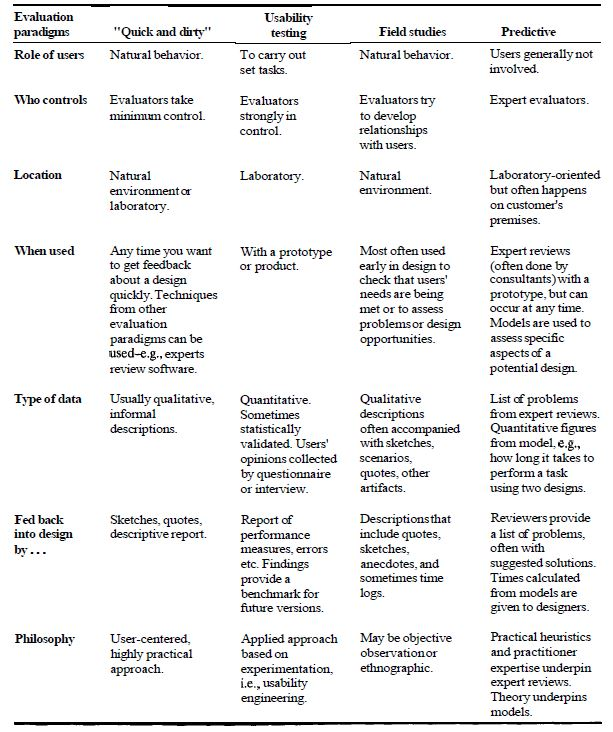
\includegraphics[width=0.90\textwidth]{figures/EvaluationParadigms.JPG}
    \caption{\label{fig:Figure_Evaluation_Paradigms}Characteristics of different evaluation paradigms}
\end{figure}
